
\documentclass[12pt]{article}
\usepackage[utf8]{inputenc}

\usepackage[a4paper, margin=1in]{geometry}

\usepackage{newtxtext}
\usepackage{amsmath,amssymb,amsthm}
\usepackage{newtxmath} % must come after amsXXX

\usepackage{float}%防止图片乱跑



\usepackage{graphicx}
%\usepackage{subfigure}




\usepackage{xcolor}
\usepackage{fancyhdr}

\usepackage{listings}
%\usepackage{ctex}

\usepackage{booktabs}


%%%%%%%%%%%% for sudocode %%%%%%%
\usepackage{algorithm}
\usepackage{algpseudocode}
%%%%%%%%%%%%%%%%%%%%%%%%%%%%%%%%%





%%%%%%%%%%%%%%%%%%%%%%%%%%%%%%%%%%%%%%%%%%%%%%%%%%%%%%%%%%%%%%%
%%%%%%%%%%%%%%%%%%%%%%%%%%%%%%%%%%%%%%%%%%%%%%%%%%%%%%%%%%%%%%%

\begin{document}

\title{530.767 CFD\\Spring 2024\\HW 1–Haobo Zhao}
\maketitle



This is CFD Homework


% \begin{figure}[H]
%     \centering
%     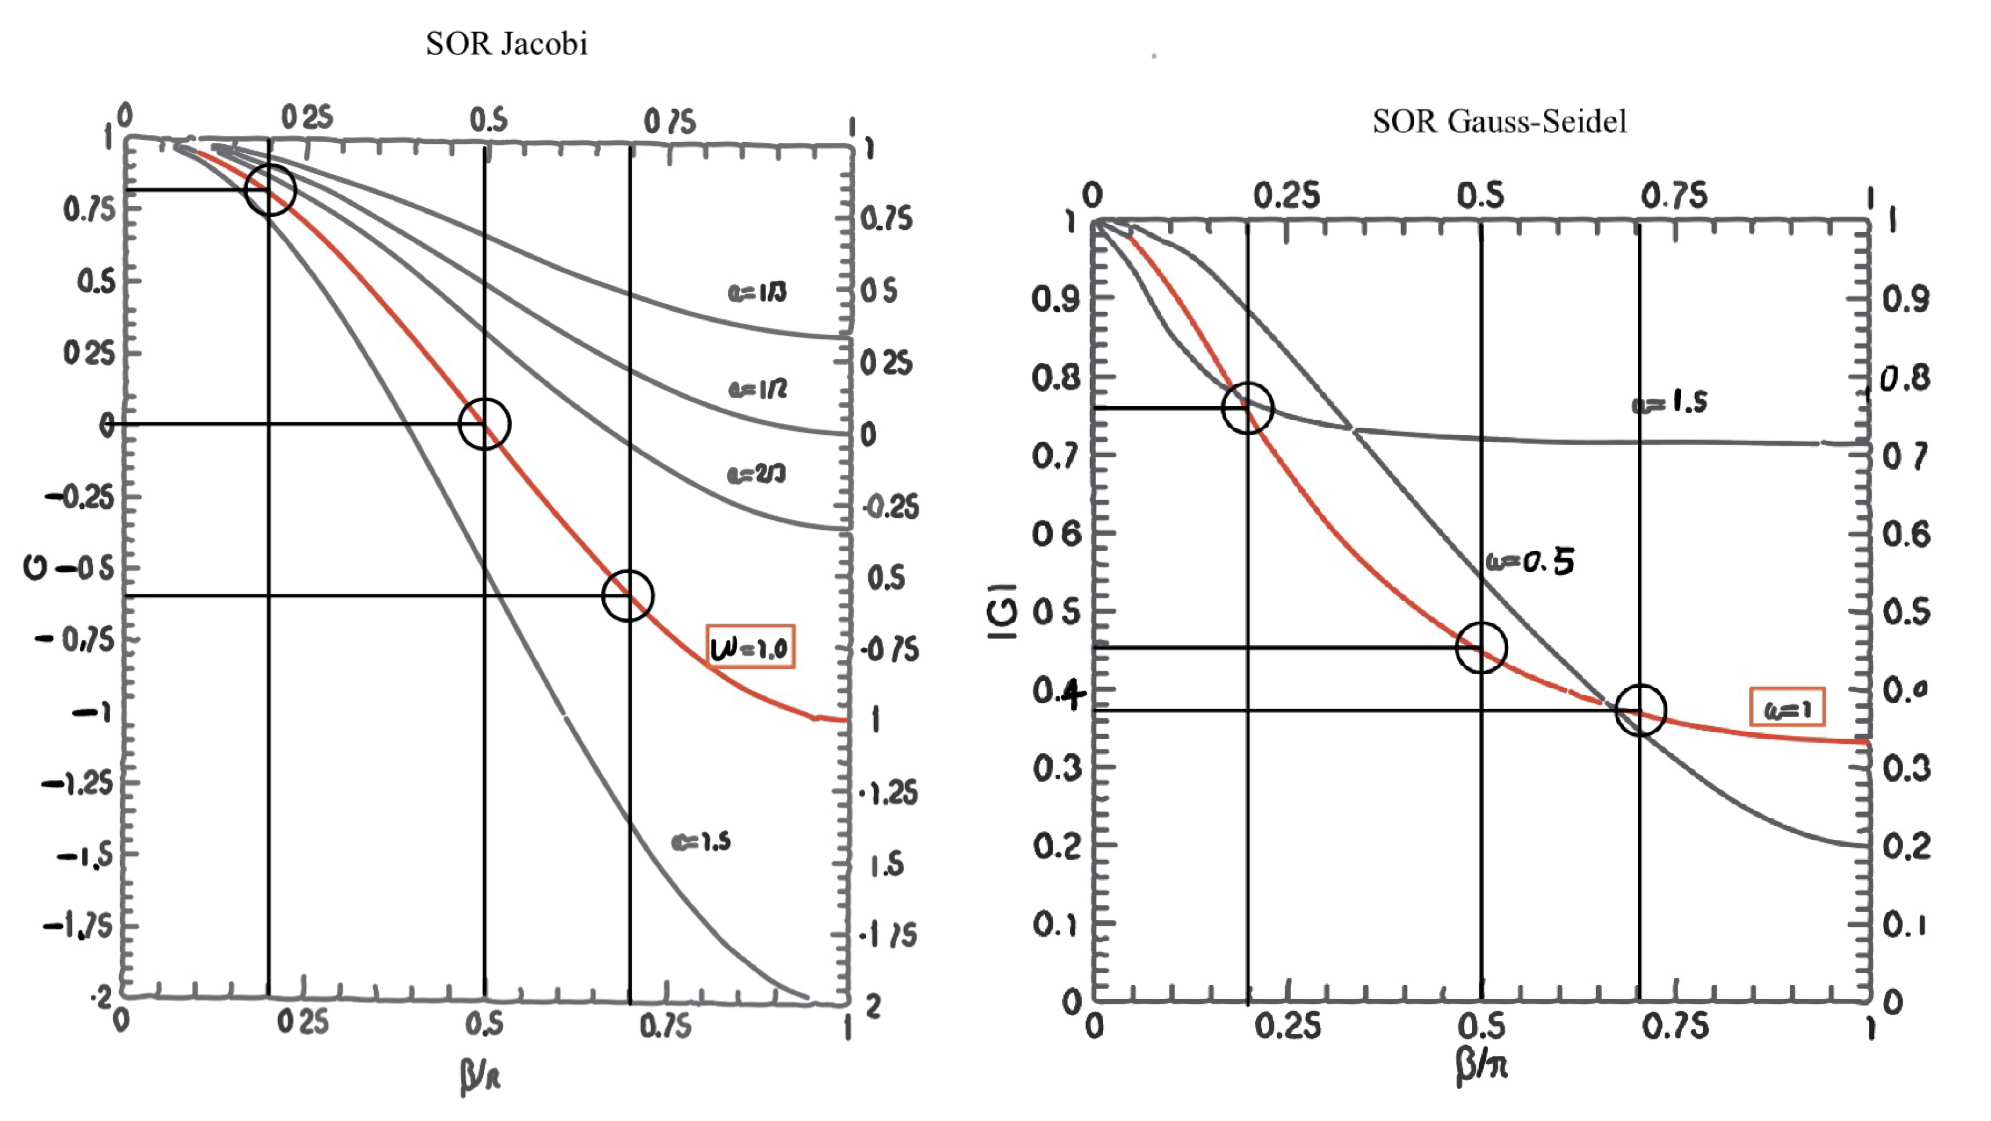
\includegraphics[width=0.8\textwidth]{IGs.jpg}
%     \label{IGs.jpg}
%     %\caption{Iteration times as k=2000, limit y in O($10^{-4}$)}
% \end{figure}


\tableofcontents


\section{Question Review}

1. We will explore the finite-difference solution to the 
simple 1-D wave equation.
Consider the following equation:
\begin{equation}
    u_t + u_x = 0; \quad \text{on} \quad 0 \leq x \leq 2\pi
\end{equation}
with
    $$u(0,t) = u(2\pi,t)$$
    $$\frac{\partial^n u}{\partial x^n} (0,t) = \frac{\partial^n u}{\partial x^n} (2\pi,t), \quad n > 0 \quad \text{(i.e. periodic BC)}$$ 
    $$u(x,0) = \sin(mx)$$

(i) Discretize the above equation with an explicit scheme 
in time on a mesh with \( \Delta x = \frac{2\pi}{20} \) 
and \( \Delta t = 0.001 \).
Use the following spatial discretization schemes:
\begin{itemize}
    \item First-order upwind
    \item Second-order upwind (using \(i, i-1, i-2\))
    \item Third order upwind (using \(i, i-1, i-2, i-3\))
    \item Third-order upwind biased (using \(i+1, i, i-1\) 
    and \(i-2\))
\end{itemize}
and obtain the numerical solution for \(m=2, 4, 6,\) 
and \(8\). You should integrate the discretized equations long 
enough in time so that the effects of the truncation error are 
apparent.\\

(ii)Derive the exact solution of the PDE.\\

(iii)Derive and plot the modified wavenumber curves 
(check the lecture notes) for the four schemes; 
use the modified wavenumber analysis to explain the observed 
behavior of the numerical solution and its comparison to the 
exact solution.\\

2. Examination of aliasing error in solutions of 
time-dependent differential equations.
Consider a domain of size \(2\pi\) and a grid
 with \( \Delta x = \frac{2\pi}{20} \) and the following 
 two equations:

    $$u_t + u^2 = 0$$
and
    $$u_t + \sin(3x)u_x = 0$$

Let the initial condition be 
\( u(x) = \sin(x) + 0.5 \sin(4x) \) and use the 
Forward Euler scheme with a time step of \(0.10\).\\

For both these equations plot and compare the unaliased 
(assuming that the aliasing error is zero) and fully aliased 
energy spectra for the resolved scales at time steps from 
\(1\) to \(10\). Explain the key characteristics of the 
results that you observe. Spectra can be obtained by running 
a FFT on your simulation results.\\

You can obtain an unaliased spectra by running the same 
simulation on a finer grid; you might also need a small 
time-step size for the finer grid.


\section{1. Finite Difference for 1D Wave Equations.}

\subsection{Finite Difference Schemes}


The PDE is showing below:

\begin{equation}
    u_t + u_x = 0; \quad \text{on} \quad 0 \leq x \leq 2\pi
\end{equation}

\subsubsection{1st Upwind Scheme}
As the equation above, the solve

\subsubsection{2nd Upwind Scheme}

\subsubsection{3rd Upwind Scheme}

\subsubsection{3rd biased Upwind Scheme}


\subsection{Solver Algorithm}

\subsection{(i) Result--Solutions for different schemes}

For the solution, the result is showing below:

For $t_{max}=0.1$, the result for different m is showing below:

\begin{figure}[H]
    \centering
    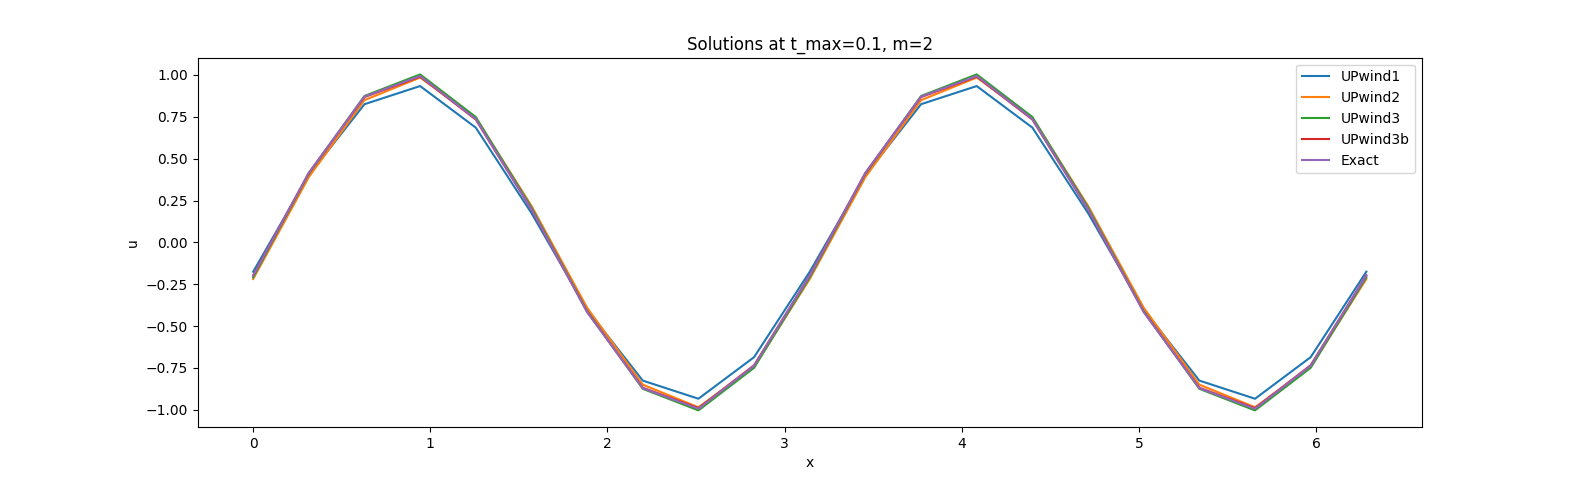
\includegraphics[width=1\textwidth]{figures/t0.1m2.png}
    \label{IGs.jpg}
    %\caption{Iteration times as k=2000, limit y in O($10^{-4}$)}
\end{figure}

\begin{figure}[H]
    \centering
    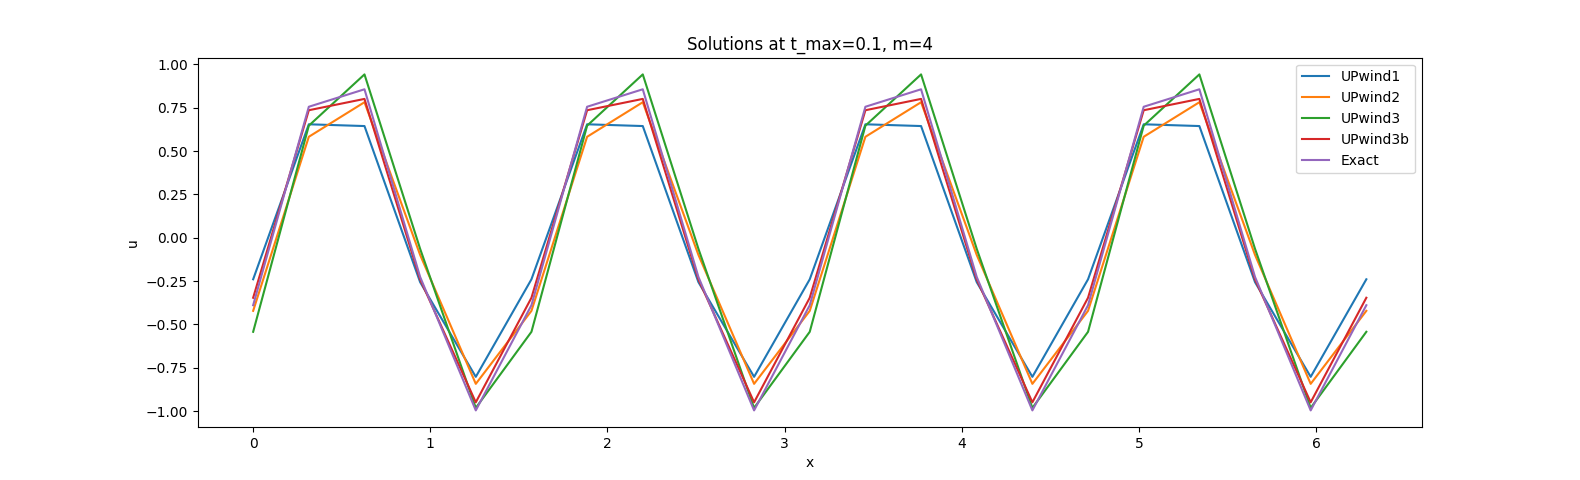
\includegraphics[width=1\textwidth]{figures/t0.1m4.png}
    \label{IGs.jpg}
    %\caption{Iteration times as k=2000, limit y in O($10^{-4}$)}
\end{figure}

\begin{figure}[H]
    \centering
    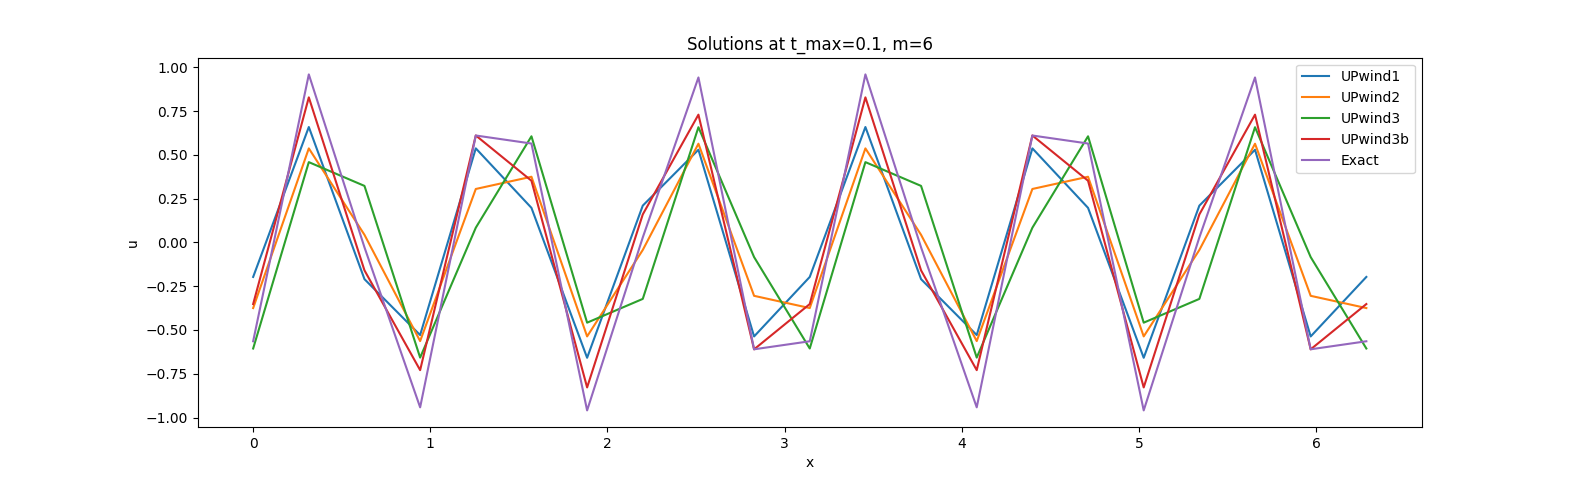
\includegraphics[width=1\textwidth]{figures/t0.1m6.png}
    \label{IGs.jpg}
    %\caption{Iteration times as k=2000, limit y in O($10^{-4}$)}
\end{figure}

\begin{figure}[H]
    \centering
    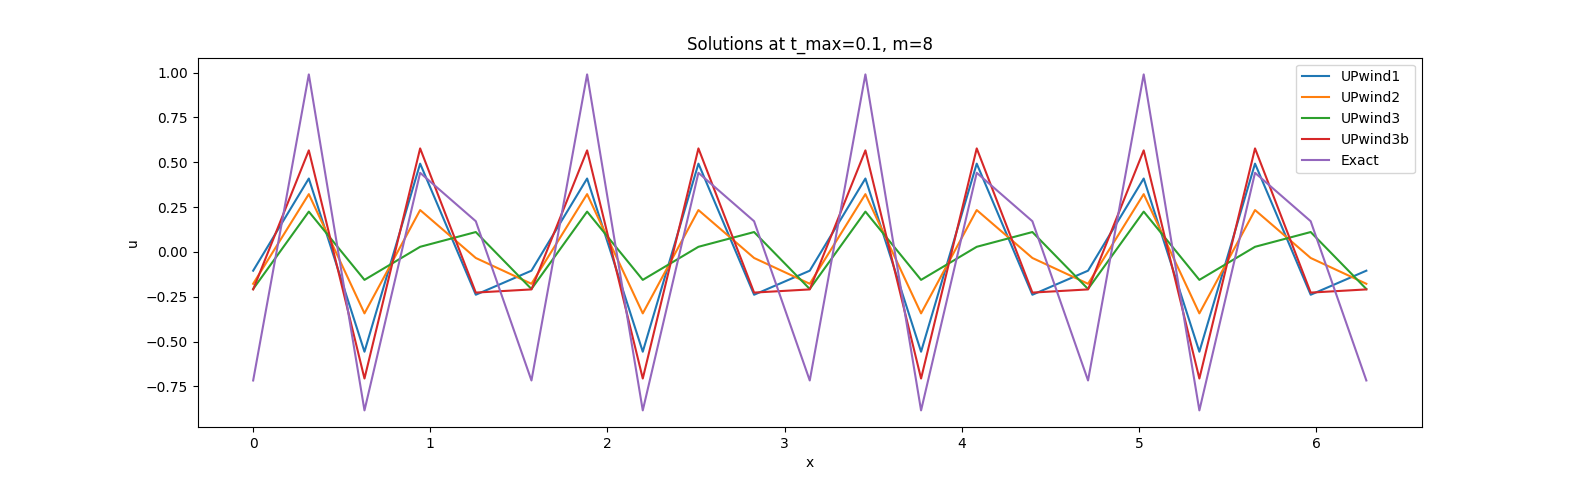
\includegraphics[width=1\textwidth]{figures/t0.1m8.png}
    \label{IGs.jpg}
    %\caption{Iteration times as k=2000, limit y in O($10^{-4}$)}
\end{figure}


For $t_{max} = 1$, the results for different m is showing below:

\begin{figure}[H]
    \centering
    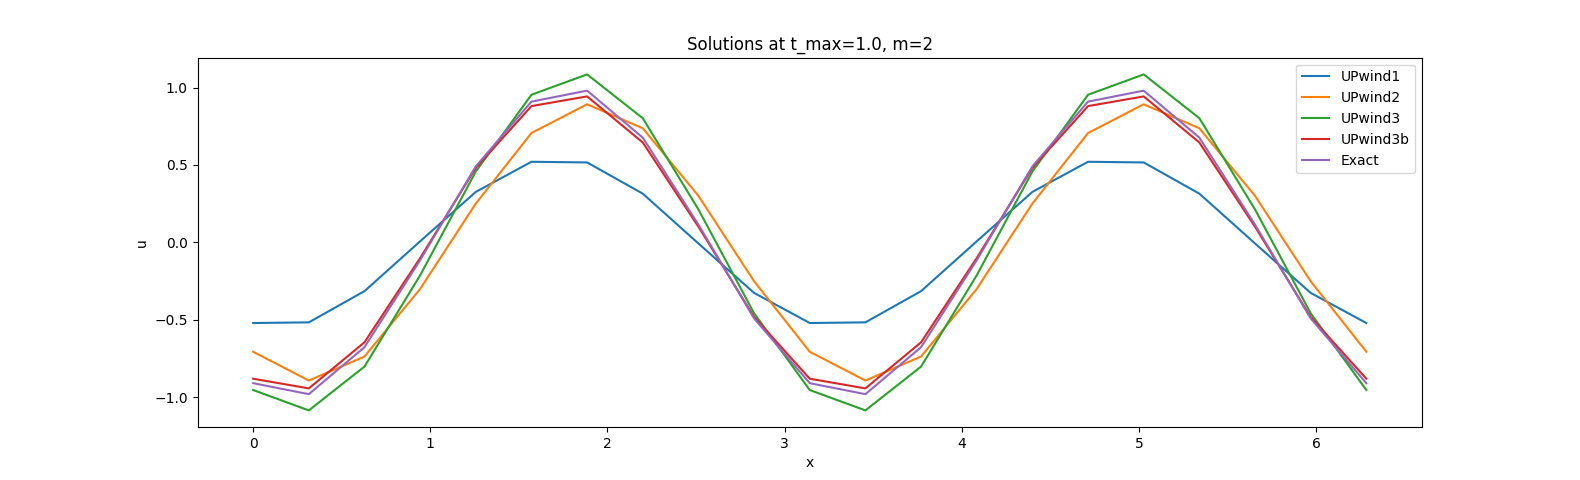
\includegraphics[width=1\textwidth]{figures/t1m2.png}
    \label{IGs.jpg}
    %\caption{Iteration times as k=2000, limit y in O($10^{-4}$)}
\end{figure}

\begin{figure}[H]
    \centering
    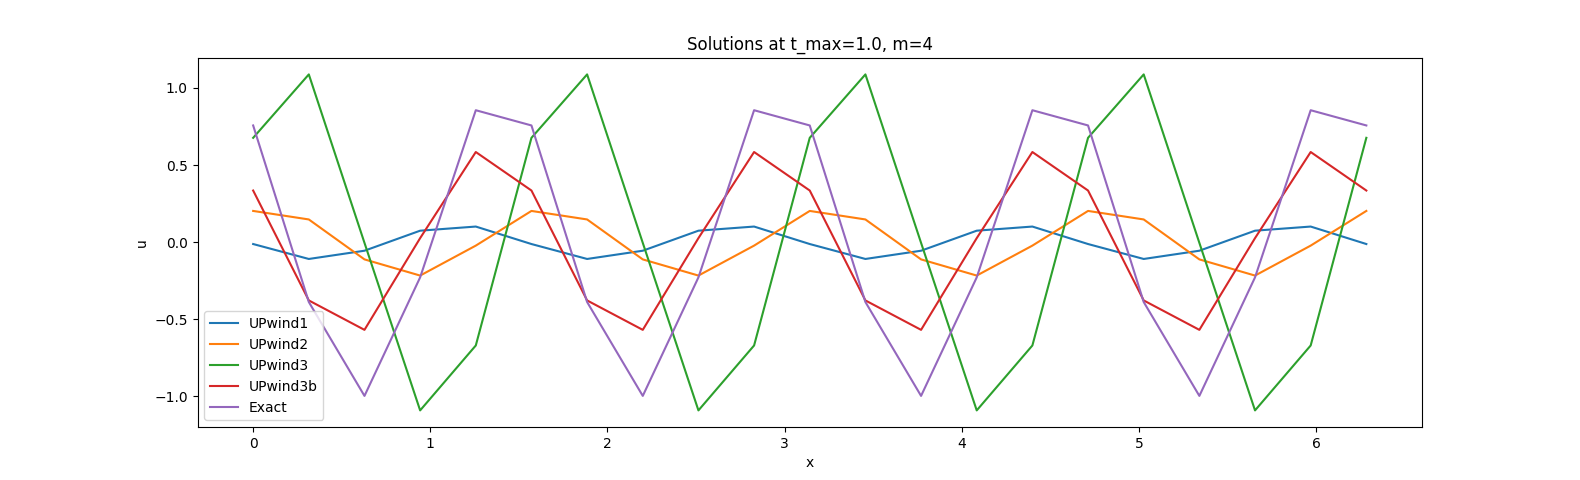
\includegraphics[width=1\textwidth]{figures/t1m4.png}
    \label{IGs.jpg}
    %\caption{Iteration times as k=2000, limit y in O($10^{-4}$)}
\end{figure}

\begin{figure}[H]
    \centering
    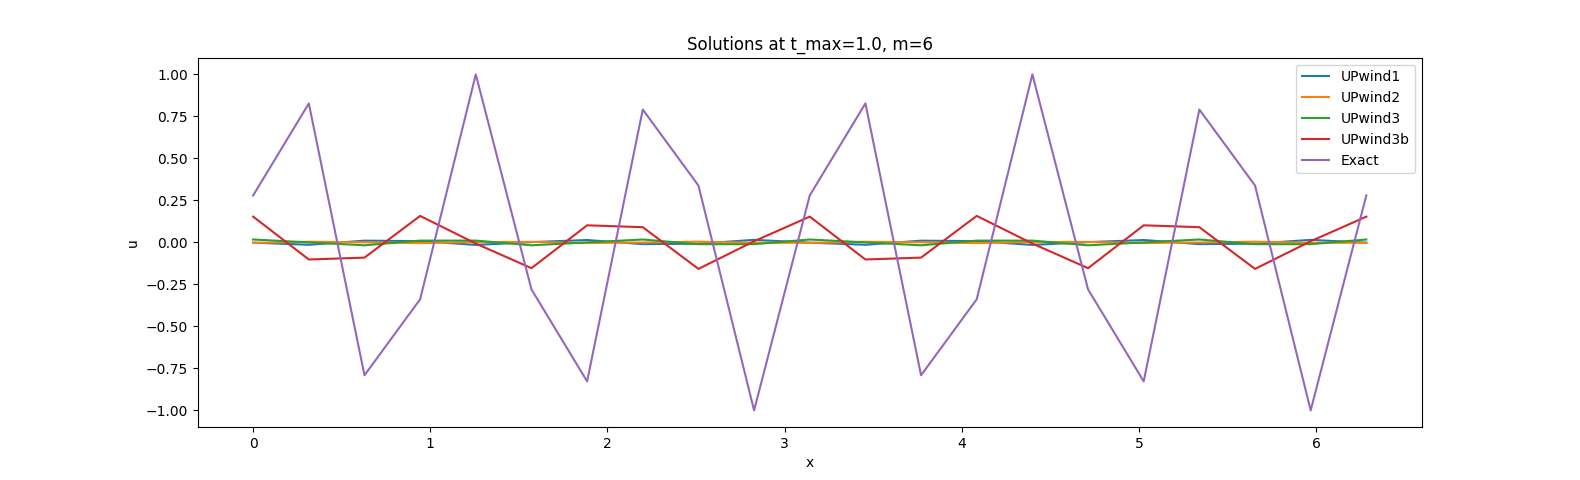
\includegraphics[width=1\textwidth]{figures/t1m6.png}
    \label{IGs.jpg}
    %\caption{Iteration times as k=2000, limit y in O($10^{-4}$)}
\end{figure}

\begin{figure}[H]
    \centering
    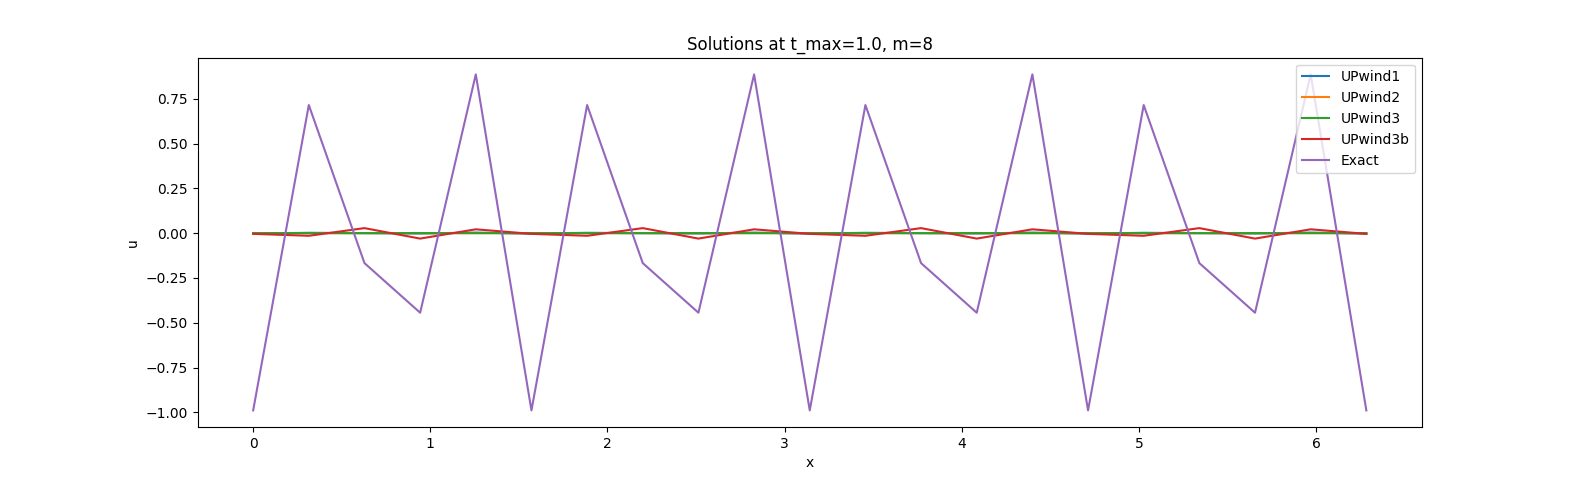
\includegraphics[width=1\textwidth]{figures/t1m8.png}
    \label{IGs.jpg}
    %\caption{Iteration times as k=2000, limit y in O($10^{-4}$)}
\end{figure}



\subsection{(ii) Exact Solution}

\subsection{(iii) Modified Wavenumber Curves and Analysis}
\subsubsection{Modified Wavenumbers}




\begin{equation}
    \begin{aligned}
    \hat{u}'_j = \frac{{u}_j - \hat{u}_{j-1}}{\Delta x} \\
    = \frac{\hat{u} e^{ikx} - \hat{u} e^{ik(x-\Delta x)}}{\Delta x} \\
    = \frac{\hat{u} e^{ikx} (1 - e^{-ik\Delta x})}{\Delta x} \\
    = \frac{\hat{u}}{\Delta x} (1 - e^{-ik\Delta x}) \hat{u} \\
    = \frac{\hat{u}}{\Delta x} \left(1 - \frac{\sin(k\Delta x/2)}{k\Delta x/2}\right) e^{ikx}
    \end{aligned}
\end{equation}
    
\begin{equation}
    \begin{aligned}
    k' = -i\left(\frac{1 - e^{-ik\Delta x}}{\Delta x}\right) = -\frac{3}{\Delta x} + i\frac{\sin(k\Delta x) + \sin(k\Delta x)}{\Delta x} = \pm \frac{\sin(k\Delta x)}{\Delta x} + i \left(\frac{\sin(k\Delta x) - 1}{\Delta x}\right)
    \end{aligned}
\end{equation}
    
    

\subsubsection{Curves and Analysis}


\begin{figure}[H]
    \centering
    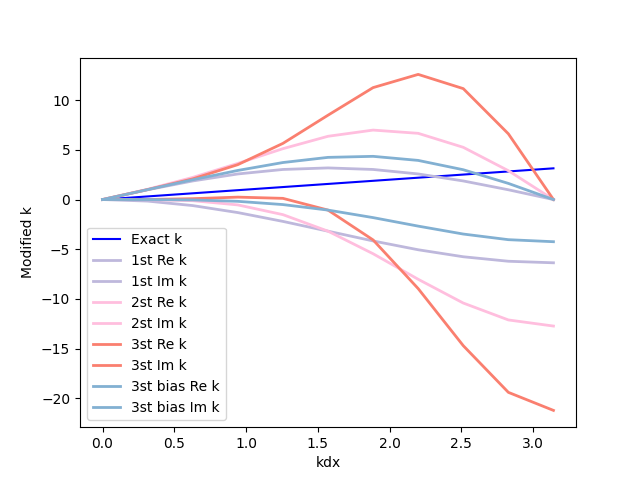
\includegraphics[width=0.8\textwidth]{figures/modifiedwavenumber.png}
    \label{IGs.jpg}
    %\caption{Iteration times as k=2000, limit y in O($10^{-4}$)}
\end{figure}

For the modified wavenumber, the result is showing above. The Exact 
wavenumber is "Exact k" in the picture, which don't have imaginary part. 
For the modified wavenumbers, each scheme's wavenumber have two parts
in the same color, the real part named "Re k" in the chart, while the 
imaginary part named "Im k" for each scheme.\\

It is easily to be observed that, for the modified wavenumber's real part,
the 3rd UPwind scheme is much larger than others, which is also far away 
from the exact k, which could explain it cannot well-simulate the equation,
espically on the lone time rigion. On the other hand, 3rd biased UPwind
scheme is much closer to the exact k than the unbiased one, which could 
explain its simulation result is closer to the exact solution.

For the modified wavenumber's imaginary part, the 3rd biased scheme's Im k
is much smaller than the others, which could explain its good simulation 
result.





\section{2. Aliased Analysis with FFT}


\begin{figure}[H]
    \centering
    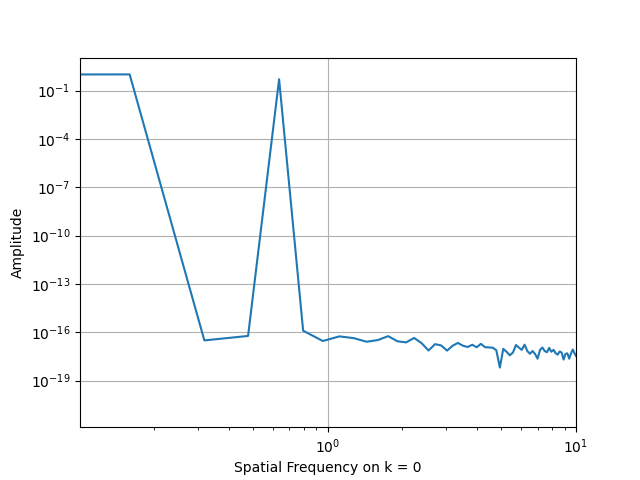
\includegraphics[width=0.45\textwidth]{figures/P2Fn1ub00.png}
    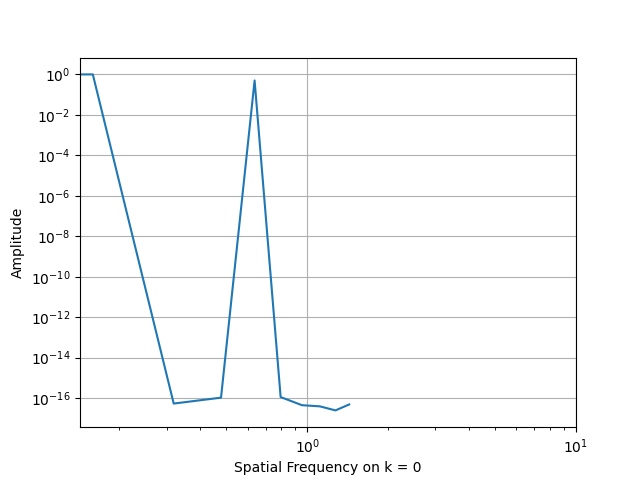
\includegraphics[width=0.45\textwidth]{figures/P2Fn1b00.png}
    \label{IGs.jpg}
    %\caption{Iteration times as k=2000, limit y in O($10^{-4}$)}
\end{figure}


\begin{figure}[H]
    \centering
    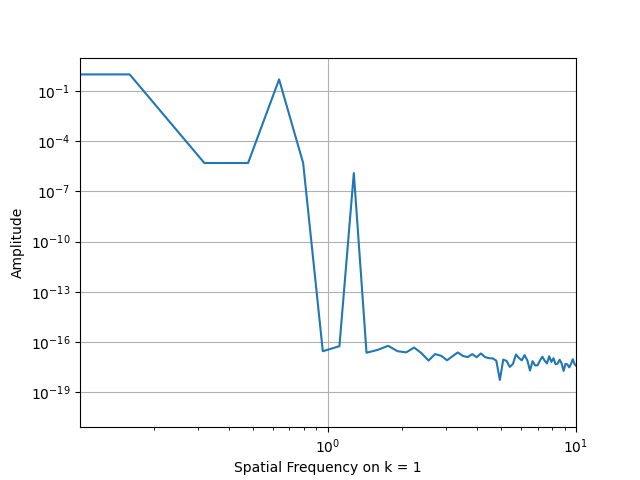
\includegraphics[width=0.45\textwidth]{figures/P2Fn1ub01.png}
    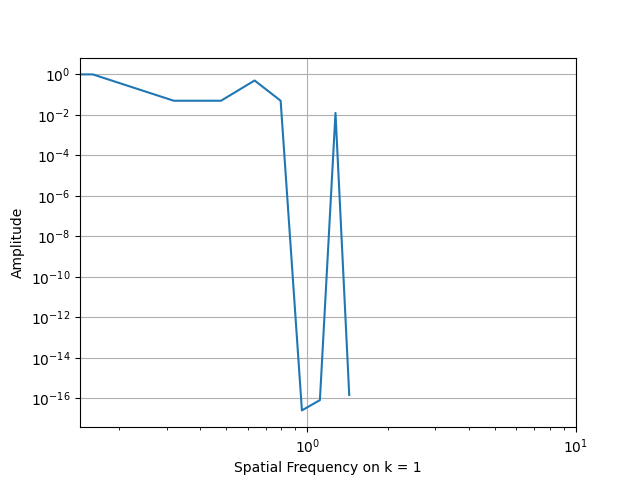
\includegraphics[width=0.45\textwidth]{figures/P2Fn1b01.png}
    \label{IGs.jpg}
    %\caption{Iteration times as k=2000, limit y in O($10^{-4}$)}
\end{figure}


\begin{figure}[H]
    \centering
    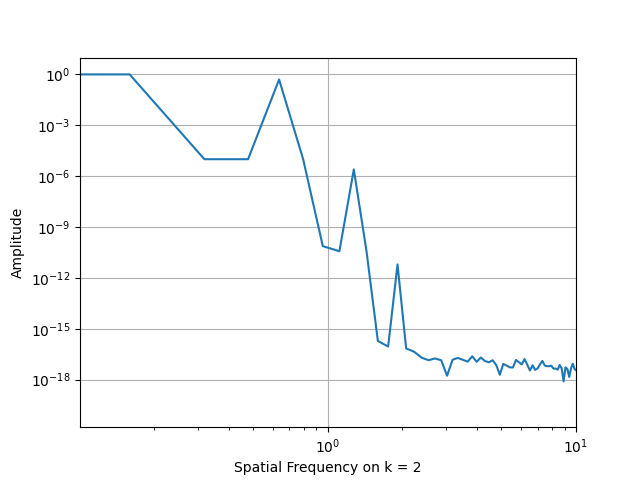
\includegraphics[width=0.45\textwidth]{figures/P2Fn1ub02.png}
    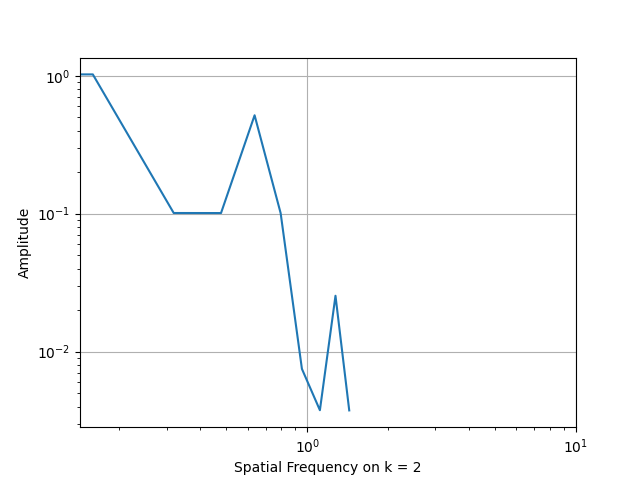
\includegraphics[width=0.45\textwidth]{figures/P2Fn1b02.png}
    \label{IGs.jpg}
    %\caption{Iteration times as k=2000, limit y in O($10^{-4}$)}
\end{figure}


\begin{figure}[H]
    \centering
    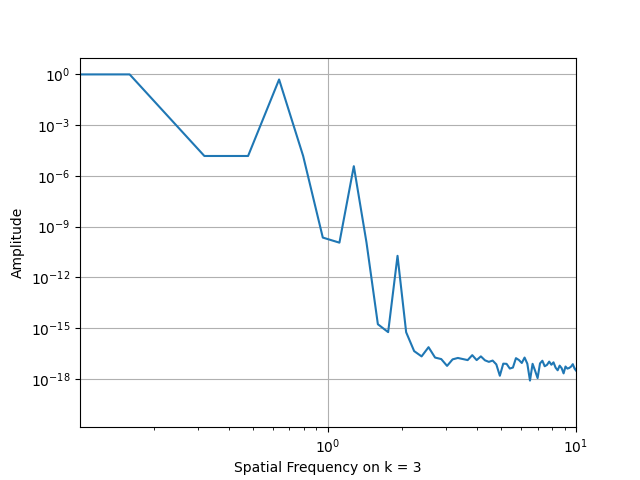
\includegraphics[width=0.45\textwidth]{figures/P2Fn1ub03.png}
    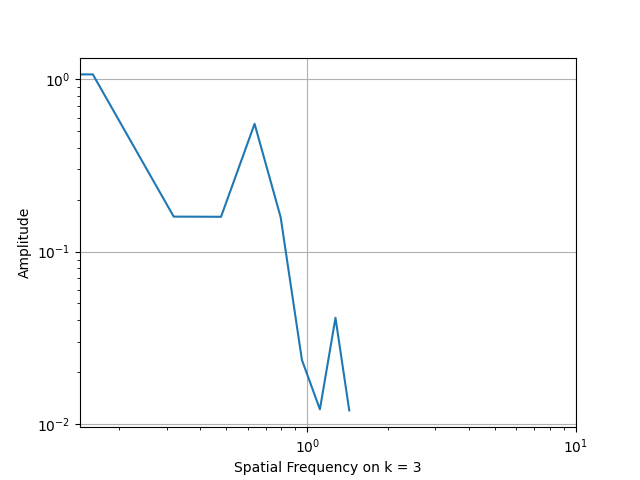
\includegraphics[width=0.45\textwidth]{figures/P2Fn1b03.png}
    \label{IGs.jpg}
    %\caption{Iteration times as k=2000, limit y in O($10^{-4}$)}
\end{figure}




\subsection{}





























%%%%%%%%%%%%%%%%%%%%%%%%%%%%%%%%%%%%%%%%%%%%%%%%%%%%%%%%%%%%%%%
%%%%%%%%%%%%%%%%%%%%%%%%%%%%%%%%%%%%%%%%%%%%%%%%%%%%%%%%%%%%%%%
%%%%%%%%%%%%%%%%%%%%%%%%%%%%%%%%%%%%%%%%%%%%%%%%%%%%%%%%%%%%%%%
\newpage
\section*{Appendix}
% 在目录中添加Appendix
\addcontentsline{toc}{section}{Appendix}
\begin{scriptsize}
\begin{lstlisting}[language=python,caption={Problem1, Py code for Solvers}]


    import math
    import numpy as np
    import matplotlib.pyplot as plt
    import matplotlib as mpl
    import copy
    
    class UPwind1st_Solver:
        def __init__(self, dx, dt, x_max, t_max,m):
            self.dx = dx
            self.dt = dt
            self.x_max = x_max
            self.t_max = t_max
    
    
            self.m = m  #added condition input
    
        def grid_generate(self):
            self.i_max = int(self.x_max/self.dx)
            self.n_max = int(self.t_max/self.dt)
    
            self.u = np.zeros(( self.i_max  ))
    
        
        def IC(self,m):
            for i in range(0, self.i_max):
                self.u[i] = math.sin(m*i*self.dx)
    
        def Iteration_Formula(self, u_W, u):
            u_new = u + (self.dt/(self.dx))*(u_W-u)
            return u_new
    
        def Iterative(self):
            u_next = copy.deepcopy(self.u)
    
            for n in range(1, self.n_max+1):
                for i in range(0,self.i_max):
                    u_next[i] = self.Iteration_Formula(self.u[i-1], self.u[i])
                self.u[:] = u_next[:]
            self.u_Full = self.getTHElastBACK(self.u)
            return self.u_Full
        
    
        def getTHElastBACK(self,u_lost):
            u_Fullget = np.copy(u_lost)
            u_Fullget = np.append(u_Fullget, [u_lost[0]])
            return u_Fullget
        
        def plot_result(self):
            x = np.arange(0,self.i_max+1)
            plt.plot(x*(2*math.pi/20),self.u_Full)
            plt.show()
    
        
        def exactsoln(self):
            u_e = np.zeros(self.i_max+1)
            for i in range(self.i_max+1):
                x = i * self.dx
                u_e[i] = math.sin(self.m * (x - self.t_max))
            return u_e
    
        def plot_result_compare(self):
            x = np.arange(0,self.i_max+1)
            u_e =  self.exactsoln()
            plt.plot(x*(2*math.pi/20),self.u_Full)
            plt.plot(x*(2*math.pi/20),u_e)
    
            print(u_e - self.u_Full)
    
            plt.show()
    
    
    
    class UPwind2nd_Solver(UPwind1st_Solver):
        def Iteration_Formula(self, u, u_W, u_WW):
            u_new = u - (3*u -4*u_W +u_WW)*self.dt/(2*self.dx)
          
            return u_new
        
        def Iterative(self):
            u_next = np.copy(self.u)
    
            for n in range(1, self.n_max+1):
                for i in range(0,self.i_max):
                    u_next[i] = self.Iteration_Formula(self.u[i],self.u[i-1],self.u[i-2])
                self.u[:] = u_next[:]
            self.u_Full = self.getTHElastBACK(self.u)
            return self.u_Full
    
    
    class UPwind3rd_Solver(UPwind1st_Solver):
        def Iteration_Formula(self, u, u_W, u_WW,u_WWW):
            u_new = u - ((11/6)*u -3*u_W +(3/2)*u_WW -(1/3)*u_WWW)*self.dt/(self.dx)
          
            return u_new
        
        def Iterative(self):
            u_next = np.copy(self.u)
    
            for n in range(1, self.n_max+1):
                for i in range(0,self.i_max):
                    u_next[i] = self.Iteration_Formula(self.u[i],self.u[i-1],self.u[i-2],self.u[i-3])
                self.u[:] = np.copy(u_next)
            
            self.u_Full = self.getTHElastBACK(np.copy(self.u))
            return self.u_Full
        
        
    
    class UPwind3rdBias_Solver(UPwind1st_Solver):
        def Iteration_Formula(self, u, u_W, u_WW,u_E):
            u_new = u - ((3)*u -6*u_W +1*u_WW +2*u_E)*self.dt/(6*self.dx)
          
            return u_new
        
        def Iterative(self):
            u_next = copy.deepcopy(self.u)
    
            for n in range(1, self.n_max+1):
                for i in range(0,self.i_max):
                    u_next[i] = self.Iteration_Formula(self.u[i],self.u[i-1],self.u[i-2],self.u[(i+1)%(self.i_max)])
                self.u[:] = u_next[:]
            self.u_Full = self.getTHElastBACK(self.u)
            return self.u_Full
        
    
    
    class Total_Compare(UPwind1st_Solver):
        def __init__(self, dx, dt, x_max, t_max, m, UPwind1, UPwind2, UPwind3, UPwind3b):
            super().__init__(dx, dt, x_max, t_max, m)
            self.UPwind1 = UPwind1
            self.UPwind2 = UPwind2
            self.UPwind3 = UPwind3
            self.UPwind3b = UPwind3b
    
        def plot_result_compare(self):
            x = np.arange(0,self.i_max+1)
    
            u_e =  self.exactsoln()
    
            plt.plot(x*(2*math.pi/20),self.UPwind1, label = "UPwind1")
            plt.plot(x*(2*math.pi/20),self.UPwind2, label = "UPwind2")
            plt.plot(x*(2*math.pi/20),self.UPwind3, label = "UPwind3")
            plt.plot(x*(2*math.pi/20),self.UPwind3b, label = "UPwind3b")
            plt.plot(x*(2*math.pi/20),u_e, label = "Exact")
    
            plt.title('Solutions at t_max=%f'%self.t_max)
            plt.xlabel('x')
            plt.ylabel('u')
            plt.legend()
            plt.show()
    

        def Error_Compute(self, u, u_e):
            Error = np.zeros(self.i_max+1)
            for i in range(0,self.i_max+1):
                    Error[i]+= abs(u[i]-u_e[i])
            return Error
    
        def plot_Error_compare(self):
            x = np.arange(0,self.i_max+1)
            u_e =  self.exactsoln()
    
            EUPwind1 = self.Error_Compute(self.UPwind1, u_e)
            EUPwind2 = self.Error_Compute(self.UPwind2, u_e)
            EUPwind3 = self.Error_Compute(self.UPwind3, u_e)
            EUPwind3b = self.Error_Compute(self.UPwind3b, u_e)
    
            plt.plot(x*(2*math.pi/20),EUPwind1, label = "UPwind1")
            plt.plot(x*(2*math.pi/20),EUPwind2, label = "UPwind2")
            plt.plot(x*(2*math.pi/20),EUPwind3, label = "UPwind3")
            plt.plot(x*(2*math.pi/20),EUPwind3b, label = "UPwind3b")
    
            plt.title('Solutions at t_max=%f'%self.t_max)
            plt.xlabel('x')
            plt.ylabel('u')
            plt.legend()
            plt.show()
    
    
    def main():
    
        x_max = 2*math.pi
        t_max = .1
    
        dx = 2*math.pi/20
        dt = 0.001
    
        m = 2
        
        
        ####### 2st Upwind Iteration
        upwind1st = UPwind1st_Solver(dx, dt, x_max, t_max,m)
        upwind1st.grid_generate()
        upwind1st.IC(m)
        U1 = upwind1st.Iterative()
    
        ####### 2nd Upwind Iteration
        upwind2nd = UPwind2nd_Solver(dx, dt, x_max, t_max,m)
        upwind2nd.grid_generate()
        upwind2nd.IC(m)
        U2 = upwind2nd.Iterative()
    
    
        ####### 3rd Upwind Iteration
        upwind3 = UPwind3rd_Solver(dx, dt, x_max, t_max, m)
        upwind3.grid_generate()
        upwind3.IC(m)
        U3 = upwind3.Iterative()
  
    
        ####### 3rd bias Iteration
        upwind3b = UPwind3rdBias_Solver(dx, dt, x_max, t_max,m)
        upwind3b.grid_generate()
        upwind3b.IC(m)
        U3b = upwind3b.Iterative()
    
    
        #### Total Compare
        Total = Total_Compare(dx, dt, x_max, t_max, m, U1, U2, U3, U3b)
        Total.grid_generate()
        Total.IC(m)
        Total.plot_result_compare()
        #Total.plot_Error_compare()
        
   
    if __name__ == '__main__':
        main()
    
    
    
\end{lstlisting}
\end{scriptsize}




%%%%%%%%%%%%%%%%%%%%%%%%%%%%%%%%%%%%%%%%%%%%%%%%%%%%%%%%%%%%%%%
%%%%%%%%%%%%%%%%%%%%%%%%%%%%%%%%%%%%%%%%%%%%%%%%%%%%%%%%%%%%%%%
%%%%%%%%%%%%%%%%%%%%%%%%%%%%%%%%%%%%%%%%%%%%%%%%%%%%%%%%%%%%%%%



\end{document}